\section{Preliminary results\label{sec:results}}
In this section the preliminary results for the stiffness of the simple Lennard--Jones system are presented. The models are to be considered as ``benchmark'' systems on which we tested our modified framework based on the CFM and with which results obtained in previous literature work are compared.

\subsection{The models}
As already explained, the CFM framework adopted allowed us to run only two independent simulations with different interface orientation. Specifically, (100) and (110) interface of an FCC crystal were chosen.

With the aim of verifying our revisited approach, we firstly studied capillary fluctuations in simple Lennard--Jones systems, leaving to future work the study of real alloy systems of concrete interest in additive manufacturing processes.

All the simulations were performed with the molecular dynamics code \textsc{lammps}, together with \textsc{plumed} for post--simulation analysis. The potential used was a truncated Lennard--Jones potential~\cite{Cheng2015}:
\begin{equation}
    \label{eqn:LJ}
    V(r)=
    \begin{cases}
        4\epsilon\left[ \left(\frac{\sigma}{r}\right)^{12} - \left( \frac{\sigma}{r}\right)^6 \right] + C_1 & r\le 2.3\sigma \\
        C_2 \left(\frac{\sigma}{r}\right)^{12}+ C_3 \left(\frac{\sigma}{r}\right)^6 + C_4 \left(\frac{\sigma}{r}\right)^2 + C_5 & 2.3\sigma < r < 2.5\sigma \\
        0 & r\ge 2.5\sigma
    \end{cases}
\end{equation}
where $C_1=0.016132\epsilon$, $C_2=3136.6\epsilon$, $C_3=-68.069\epsilon$, $C_4=-0.083312\epsilon$ and $C_5=0.74689\epsilon$. The timestep was set equal to 0.004 time units in the Lennard--Jones scheme. The direction parallel to the interface normal was aligned with the $z$ axis and throughout all the simulations the $NP_zT$ ensemble was employed, with the Nose--Hoover thermostat and barostat to control pressure and temperature of the system.

The simulations for both the interfaces studied were run at the equilibrium melting temperature of 0.618 (in LJ units) and the initial crystalline systems were prepared considering the equilibrium lattice parameter at that temperature.

Models of both solid--liquid interfaces studied were generated as follows: once the interface of interest had been fixed, a perfect crystalline FCC unit cell was prepared with a lattice parameter consistent with the chosen temperature ($T_m$). The $z$ axis of the coordinate system was always aligned with the direction indicating the interface normal. Then, the unit cell has been replicated in the $xy$ plane and along $z$, always with a larger number of replicas in the $z$ direction, to ensure that solid and liquid regions were not too thin and statistical fluctuations too large.

First step of the simulations was actually generating the solid--liquid interface. To this end, a central slab of atoms has been held fixed: the size of this region depended on the length of the supercell in the $z$ direction (between $L_z/3$ and $2L_z/3$). A number of simulation steps ($\approx \num{25e3}$) were run in $NPT$ ensemble with the temperature fixed well above $T_m$, leading to complete melting of the two side regions of the supercell. Afterwards, the same number of steps were run with the target temperature of the thermostat being again fixed at $T_m$ and then a number of equilibration steps was carried out, letting all the atoms follow the unconstrained dynamics. With the protocol described, after approximately \num{1e5} MD steps, we obtained the equilibrated systems at the melting temperature with coexistence of solid and liquid regions. It is worth noting that no adjustment of the density was necessary when the liquid parts were generated, because the pressure was kept constant by the barostat and the volume was always free to fluctuate.



\subsection{(100) interface}
Following the recipe described above, to study (100) interface a supercell of $20\times 20 \times 50$ unit cells (in $x$, $y$ and $z$ direction respectively) was generated. The total number of atoms is \num{80000}. Since for an FCC crystal directions in direct space $[hkl]$ is perpendicular to the surface with the same Miller indexes\footnote{This statement is in general true for Bravais lattices with equal length basis vectors.}, the crystallographic axes were aligned along the standard Cartesian coordinate system.

\subsubsection{Grid spacing and bandwidth}
As the (100) model was the first to be studied, we ran preliminary tests changing the two tunable parameters when computing the order parameter field of \cref{eqn:op-field2}: the coarse--graining length $\xi$ and the spacing of the grid on which all the distances appearing in \cref{eqn:op-field2} were computed\footnote{In \cref{eqn:op-field2} the symbol $\bm{r}$ denotes an arbitrary position with respect to a chosen coordinate system. It is clear that, when computing the distance term in that expression, only a finite set of points in space can be ``sampled'': these points are those of a regular 3D grid, built considering the simulation box sizes and the spacing between two consecutive points in each direction.}.

For the grid spacing, we analysed the same trajectory of \num{1e6} steps (not counting the steps carried out for preparing the model, as described above) with the following different grid spacings: \numlist{0.25;0.5;1.0} (in LJ distance units). We noticed that only \num{1.0} gave an appreciable difference in the Fourier spectrum. This parameter controls the total number of grid points (and in turn the number of $k$ points, but not the smallest wave vector possible, which depends only on the simulation cell size), so a smaller value would mean having just more points for which to compute the distances with all the atoms; a value chosen within a reasonable range\footnote{``Big'' is far from specific, obviously: we can say that big would mean choosing a value much larger than the average distance between atoms; this choice would lead to a very coarse grid poorly sampling the simulation box.} does not affect much the result (i.e.\ the Fourier spectrum). For this reason, all the analysis were done with a grid spacing of \num{0.5}, a value that even for large simulation cells did not result in too expensive calculations.

The coarse--graining length (or bandwidth) $\xi$ deserves more attention, because this parameter also enters the model used afterwards to fit the Fourier spectrum and obtain the stiffness tensor.
We recall that the original model used for the fits is something like $A(k) \propto 1/k^2$, while our model has a multiplicative Gaussian term in addition: $A(k) \propto \exp{(-k^2/2\sigma_k^2)}/k^2$. As we built our order parameter density field by means of a convolution, Fourier transforming a Gaussian gives another Gaussian in $k$ space with the only difference in the bandwidth. Specifically, it holds the relation $\sigma_k = 1/\sigma$. Thus, we expect that a change in the $\xi$ used to build the coarse--grain field will influence the region of $k$ space over which the Gaussian smoothening shows its effect; in particular, the larger $\xi$, the narrower this region will be. As \cref{fig:bandwidths} shows, this is exactly what we obtained.
\begin{figure}[tb]
    \centering
    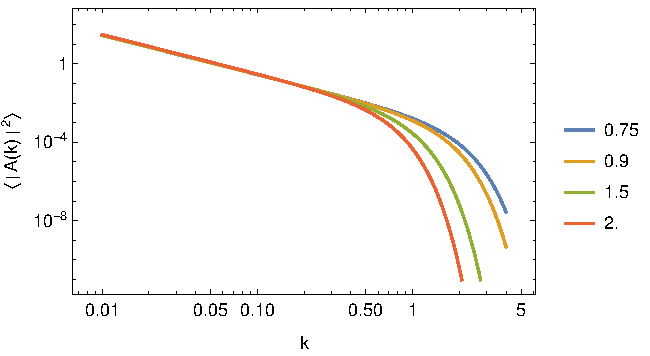
\includegraphics[width=.7\textwidth]{bandwidthComparison}
    \caption{Plots of the fitted Fourier spectrum with different values of $\xi$ used to build the coarse--grained field. Here $k$ stands for $k_x$.}
    \label{fig:bandwidths}
\end{figure}


\subsubsection{Computing the average Fourier spectrum}
As explained in \cref{sec:method}, the quantity subject to the fit as a function of $\bm{k}$ vectors is the average Fourier spectrum, $\langle |A(k_x,k_y)|^2 \rangle$. The easiest approach to compute this quantity, assuming valid the ergodicity postulate, would be to calculate for each $\bm{k}$ vector the time average of the corresponding Fourier amplitude (the square modulus of it). With this average it is also straightforward to compute the standard error of the mean.

The problem arises when dealing with time correlated data. Since we are studying fluctuations in Fourier spectrum, $\langle |A(\bm{k},t)|^2 \rangle$ is a clear example of data correlated in time. There are many ways to compute the correct error estimate of data of this kind. The main one consists of computing the so--called time auto--correlation function of the data set; the problem is that computing time correlation functions is usually expensive and requires a very frequent sampling (on the time scale) of the data. Another way of estimating statistical errors is studying the behaviour of so--called block averages~\cite{FrenkelSmitMD}.

What we did is a sort of combination of these two methods: since computing the time correlation function for every $\bm{k}$ point would have been too expensive, we considered only those $\bm{k}$ vectors with a zero component, namely $(2\pi j_x/L_x,0)$ and $(0,2\pi j_y/L_y)$. We then calculated the fundamental quantity of auto--correlation time, $\tau$, which gives an estimate of how long one would have to ``wait'' between two consecutive samples of the measured observable to collect uncorrelated measures of it. Then, we used this information to compute the proper average and corrected error following the ``block average'' algorithm.

The idea of the block average is the following~\cite{Flyvbjerg1989}: let $A_1,A_2,\dots,A_L$ be $L$ consecutive samples of the quantity we want to calculate the average and its error. We now group our data in the following way
\begin{equation}
    A'_i= (A_{2i-1}+A_{2i})/2
\end{equation}
with $L'=0.5 L$. Clearly, the average of this ``new'' set of data is unchanged. The variance of this new set is given by
\begin{equation}
    \sigma^2(A')=\langle A'^2 \rangle - \langle A'\rangle^2=\frac{1}{L'}\sum_{i=1}^{L'} A'^2_i-\bar{A}'^2_i.
\end{equation}
If we perform again this blocking operation (taking instead of couple of data, group of three) and if we have a simulation long enough, the averages $A'_i$ will become completely uncorrelated. This means that the following relation would hold
\begin{equation}
    \frac{\sigma^2(A')}{L'-1}\approx \text{constant}.
\end{equation}
In a similar way, we can also determine the statistical error of $\sigma^2(A')$, which would give an estimate of the variance in our ensemble average
\begin{equation}
\label{eqn:error-blocked}
    \sigma^2(A) \approx \frac{\sigma^2(A')}{L'-1} \pm \sqrt{\frac{2\sigma^4(A')}{(L'-1)^3}}.
\end{equation}
In our case, we have also an estimate of what is the auto--correlation time $\tau$, so we can avoid the full block average calculation and compute the error given by \cref{eqn:error-blocked} with a block size $L'$ corresponding to a time interval of $\sim \tau$. In this way the final ensemble average will have an error estimate appropriately adjusted taking into account time correlation.

\subsubsection{Stiffness tensor for (100)}
Having explained all the technical details, we present in this section the results for the stiffness tensor obtained in our simulations. According to the analysis explained in the previous section, the average of the Fourier spectrum and its error estimates were computed considering blocks of 72 frames.

Since (100) is a highly symmetric surface for the FCC system, it can be shown that the following relations hold for the stiffness tensor, $\sigma$: $\sigma_{11}=\sigma_{22}$ and $\sigma_{12}$ is zero. \Cref{tab:stiffness} summarizes the results obtained and compares them with the values of~\textcite{Becker2009:CFM2D}\footnote{In this work, the fitting model is a symmetry--consistent model, that is for the (100) only one value of the stiffness tensor was considered. The model is identical to the one used for one--dimensional interfaces.}.
\begin{table}[tb]
    \centering
    \caption{Stiffness values calculated by our method at \num{0.6185} reduced temperature for (100) and (110) interfaces. Units on stiffness are $(\epsilon/\sigma^2)$. The values obtained by Becker at the same temperature are also reported for comparison (95\% confidence level on the last digit).}
    \begin{tabular}{lccccc}
        \toprule
        \multirow{2}*{Interface  $(hkl)$} & \multicolumn{3}{c}{Present work} & \multicolumn{2}{c}{Ref.~\cite{Becker2009:CFM2D}}\\
        \cmidrule(r){2-4}\cmidrule(l){5-6}
        & $\sigma_{11}$ & $\sigma_{22}$ & $\sigma_{12}$ & $\sigma_{11}$ & $\sigma_{22}$\\
        \midrule
        $(100)$ & $0.2897\pm \num{8.0e-4}$ & $0.2871\pm \num{7.0e-4}$ &\num{4.6e-18} & \num{0.2866} & -- \\
        $(110)$ & $\num{0.379}\pm \num{1.0e-3}$  & $\num{0.316}\pm \num{1.0e-3} $ & \num{1.13e-19} & \num{0.431} & \num{0.305} \\
         \bottomrule
    \end{tabular}
    \label{tab:stiffness}
\end{table}




\subsection{(110) interface}
The model used to study (110) interface was prepared in the same way as the one for the (100); the only differences are the number of unit cells for each direction of the supercell ($20\times 20\times 30$) and the directions along which the Cartesian axes where aligned: $x$ axis is along $[\bar{1}10]$, $y$ along $[001]$ and $z$ along $[110]$, that is the normal to the interface $(110)$. Incidentally, this is the same configuration adopted by~\textcite{Becker2009:CFM2D}. The results obtained for the stiffness tensor are reported in \cref{tab:stiffness}. In this case, average of the Fourier spectrum was computed with block of 6 frames.